%----------------------------------------------------------------------------
\chapter{Mérési feladatok}\label{sect:LatexTools}
%----------------------------------------------------------------------------
%
%\begin{figure}[!ht]
%	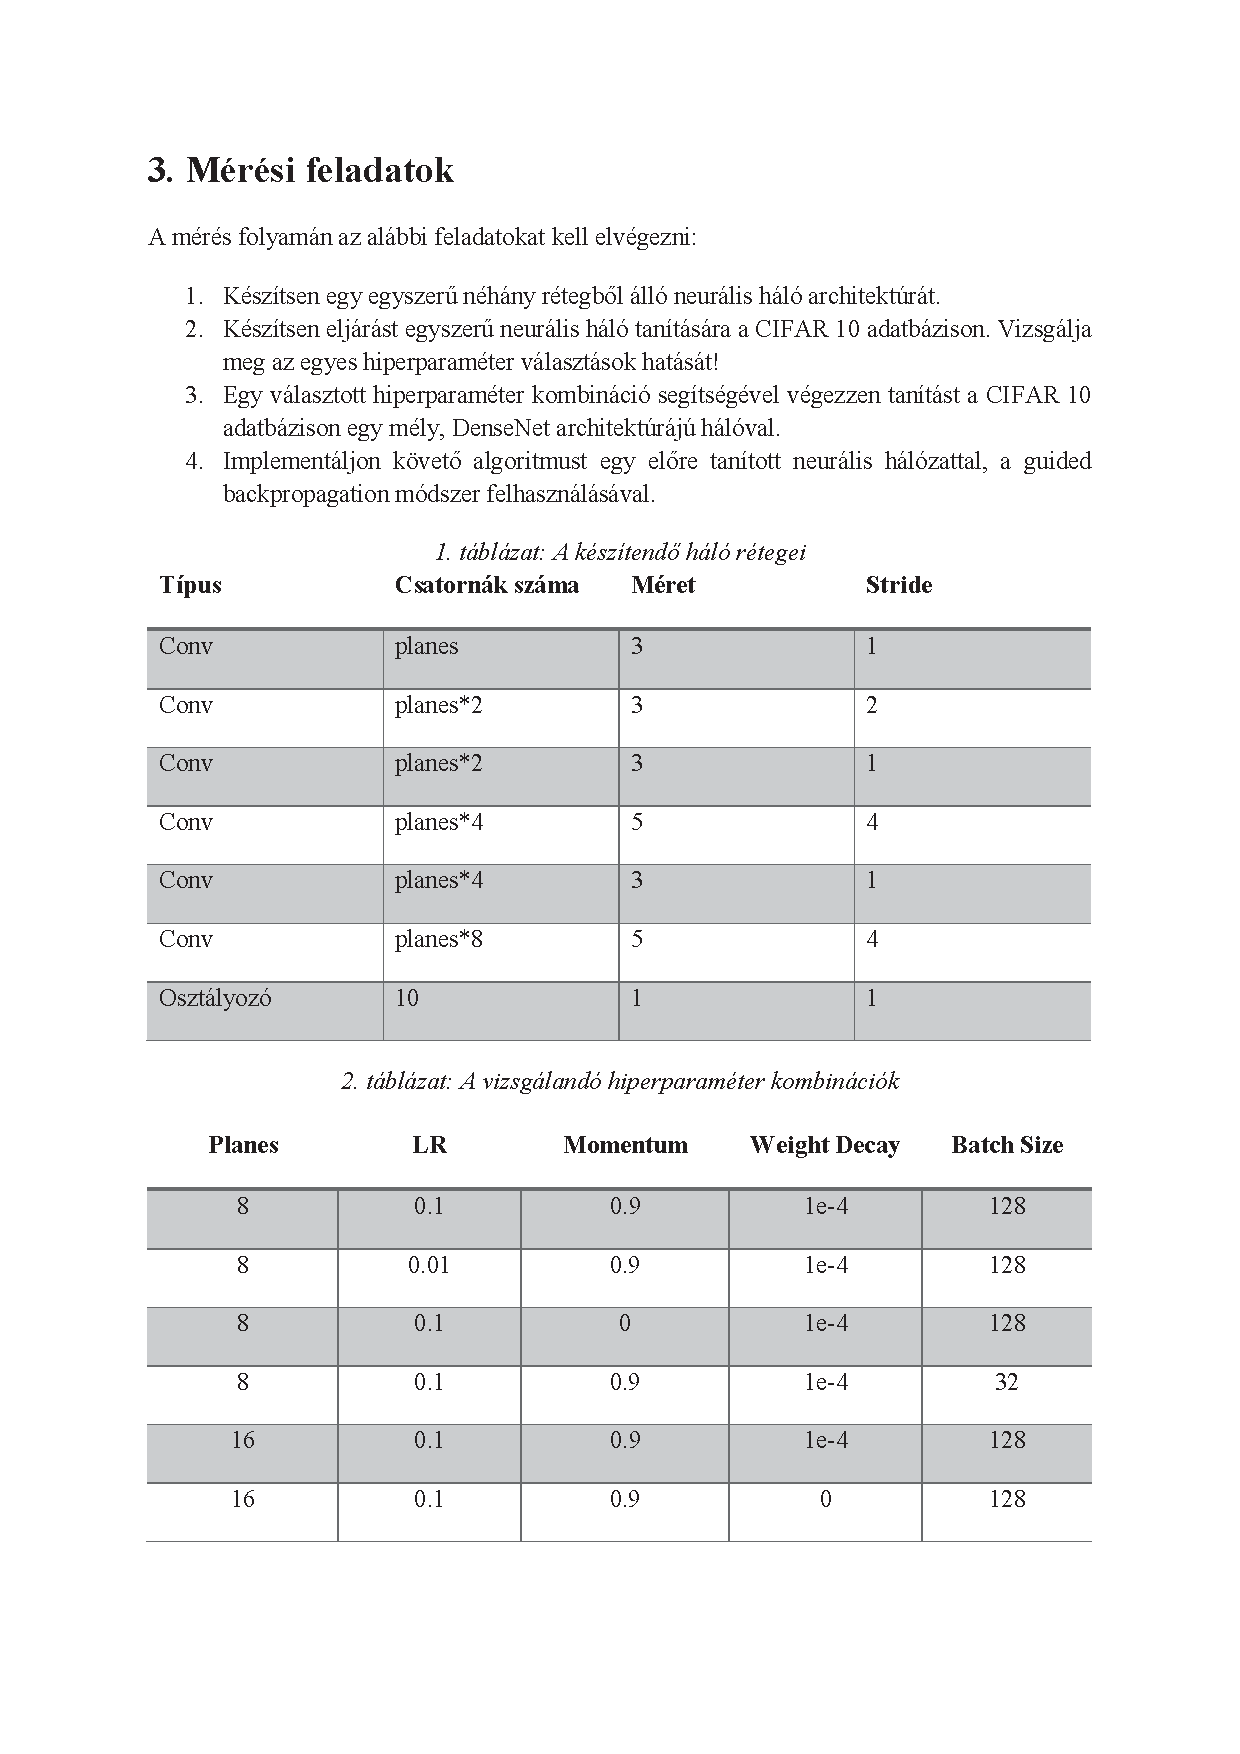
\includegraphics[trim = 25mm 210mm 20mm 33mm,clip, width=150mm,keepaspectratio]{figures/feladatok_m07.pdf}
%	\label{fig:Road-of-a-char}
%\end{figure}

A mérés folyamán az alábbi feladatokat kell elvégezni:
\begin{enumerate}
	\item Végezze el a tervezést a Matlab segítségével és vizsgálja meg a tranzienseket a Simulinkben megvalósított
	modell segítségével!
	\item Módosítsa a bizonytalan paramétereket a mérésvezető által megadott paraméterekre és vizsgálja meg
	a tranzienseket!
	\item Végezze el a robusztus szabályozók újratervezését módosított előírt viselkedés (modell) esetén és
	vizsgálja meg a tranzienseket!
	\item Más bizonytalansági paraméter intervallumok mellett módosítsa a DW súlyozó mátrix elemeit, majd
	tervezze újra a szabályozót és vizsgálja meg az időtartománybeli tranziensek minőségét!
\end{enumerate}
